\documentclass{article}
\usepackage{geometry}  
\usepackage{amsmath}  
\usepackage{graphicx} 
\usepackage{svg}
\usepackage[T1]{fontenc}
\usepackage{float}
\usepackage[utf8]{inputenc}

%----------------------------------------------------------------------------------------
%	REPORT INFORMATION
%----------------------------------------------------------------------------------------

\title{TRA - Techniki Realizacji Algorytmów Cyfrowego Przetwarzania Sygnałów  \\ Projekt -badanie modulacji PWM i PDM na wejściu wzmacniacza D klasy - specyfikacja końcowa \\} % Report title

\author{Anna \textsc{Dzieżyk}, indeks: 318506 \\ }% Author name(s), add additional authors like: '\& James \textsc{Smith}'

\date{\today} % Date of the report

%----------------------------------------------------------------------------------------

\begin{document}

\maketitle % Insert the title, author and date using the information specified above
\section{Wstęp}
Założeniem projektu jest porównnaie działania wzmacniacza klasy D, używanego często do zastosowań audio, gdzie 
rozdzielczość sygnału jest ważna, z różnymi stopniami wejściowymi. Badane stopnie wejściowe to będą: komparator oraz przetwornik sigma delta pierwszego rzędu. 
\\
Niestety założenia zaimplemenotwania projektu całkowicie teoretycznie nie zostały do końca spełnione - zostały wykonane dwie realizacje wzmacniacza klasy D w porgramie LTSpice, bez wykonywania modułów w matlabie.
Wadą tego rozwiazania jest fakt, że nie możemy dokładnie zbadać wrażliwości obydwu układów na szumy sygnału wejciowego, niosącego informację, za to bardziej dokładnie odtwarzamy zachowanie
tychże układów zbudowanych z rzeczywistych układów scalonych.

\section{Badane układy}
\subsection{Schematy elektryczne}
\begin{figure} [H]
	\centering
	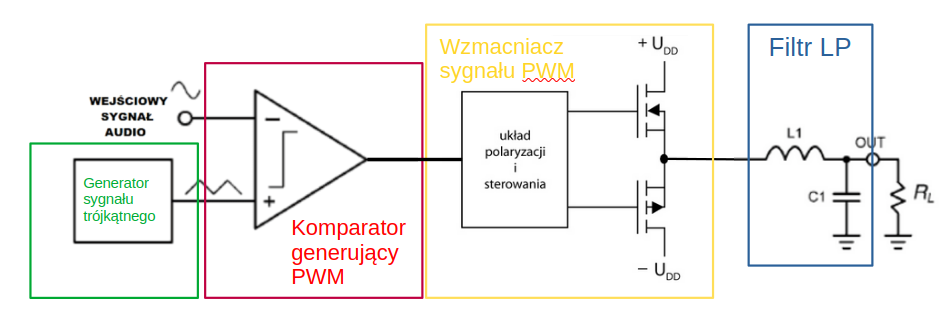
\includegraphics[scale=0.5]{block_digram_class_d_comp.png}
	\caption{Schemat blokowy całego typowego wzmacniacza klasy D z komparatorem generującym przebieg PWM}
 \end{figure}
 
 \begin{figure} [H]
	\centering
	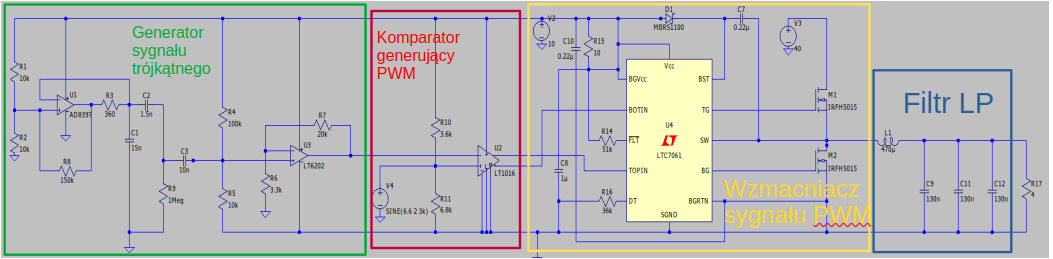
\includegraphics[width = \textwidth]{schemat_d_Class_comp.png}
	\caption{Schemat elektryczny badanego wzmacniacza klasy D z komparatorem generującym przebieg PWM}
 \end{figure}

 \begin{figure} [H]
	\centering
	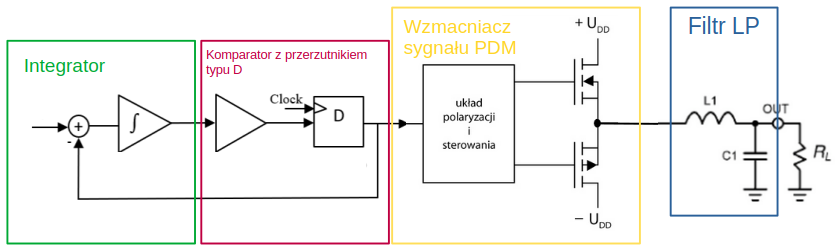
\includegraphics[scale=0.5]{block_diagram_class_d_sigmadelta.png}
	\caption{Schemat blokowy całego typowego wzmacniacza klasy D z modulatorem sigma-delta generującym przebieg PWM}
 \end{figure}

 \begin{figure} [H]
	\centering
	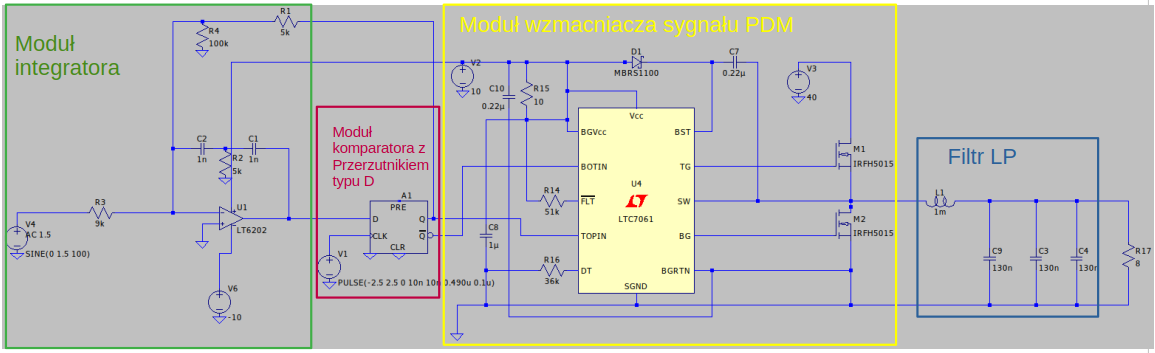
\includegraphics[width = \textwidth]{schemat_d_Class_sigma_delta.png}
	\caption{Schemat elektryczny badanego wzmacniacza klasy D z modulatorem sigma-delta generującym przebieg PDM}
 \end{figure}
\subsection{Testy niskich częstotliwości $f_{in} = 100Hz.$}
\begin{figure} [H]
	\centering
	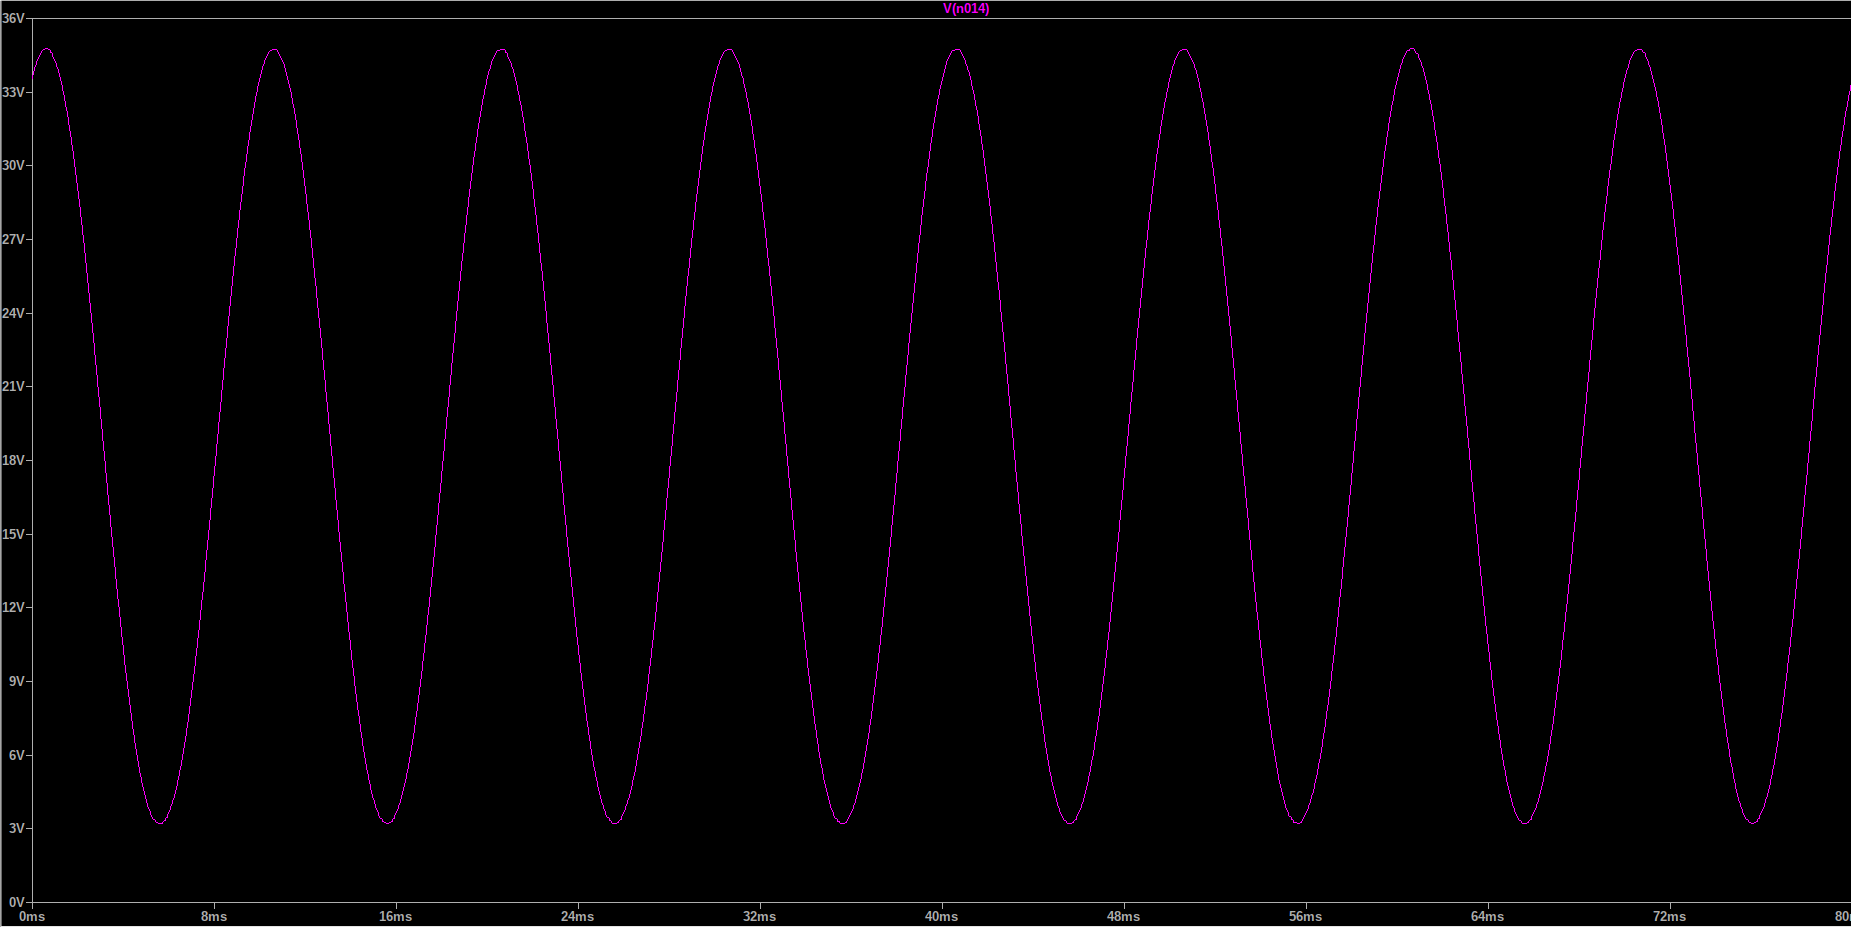
\includegraphics[width = \textwidth]{Vout_comp_100hz.png}
	\caption{Sygnał odtworzony z sygnału sygnału PWM ze wzmacniacza klasy d z komparatorem}
 \end{figure}
 
 \begin{figure} [H]
	\centering
	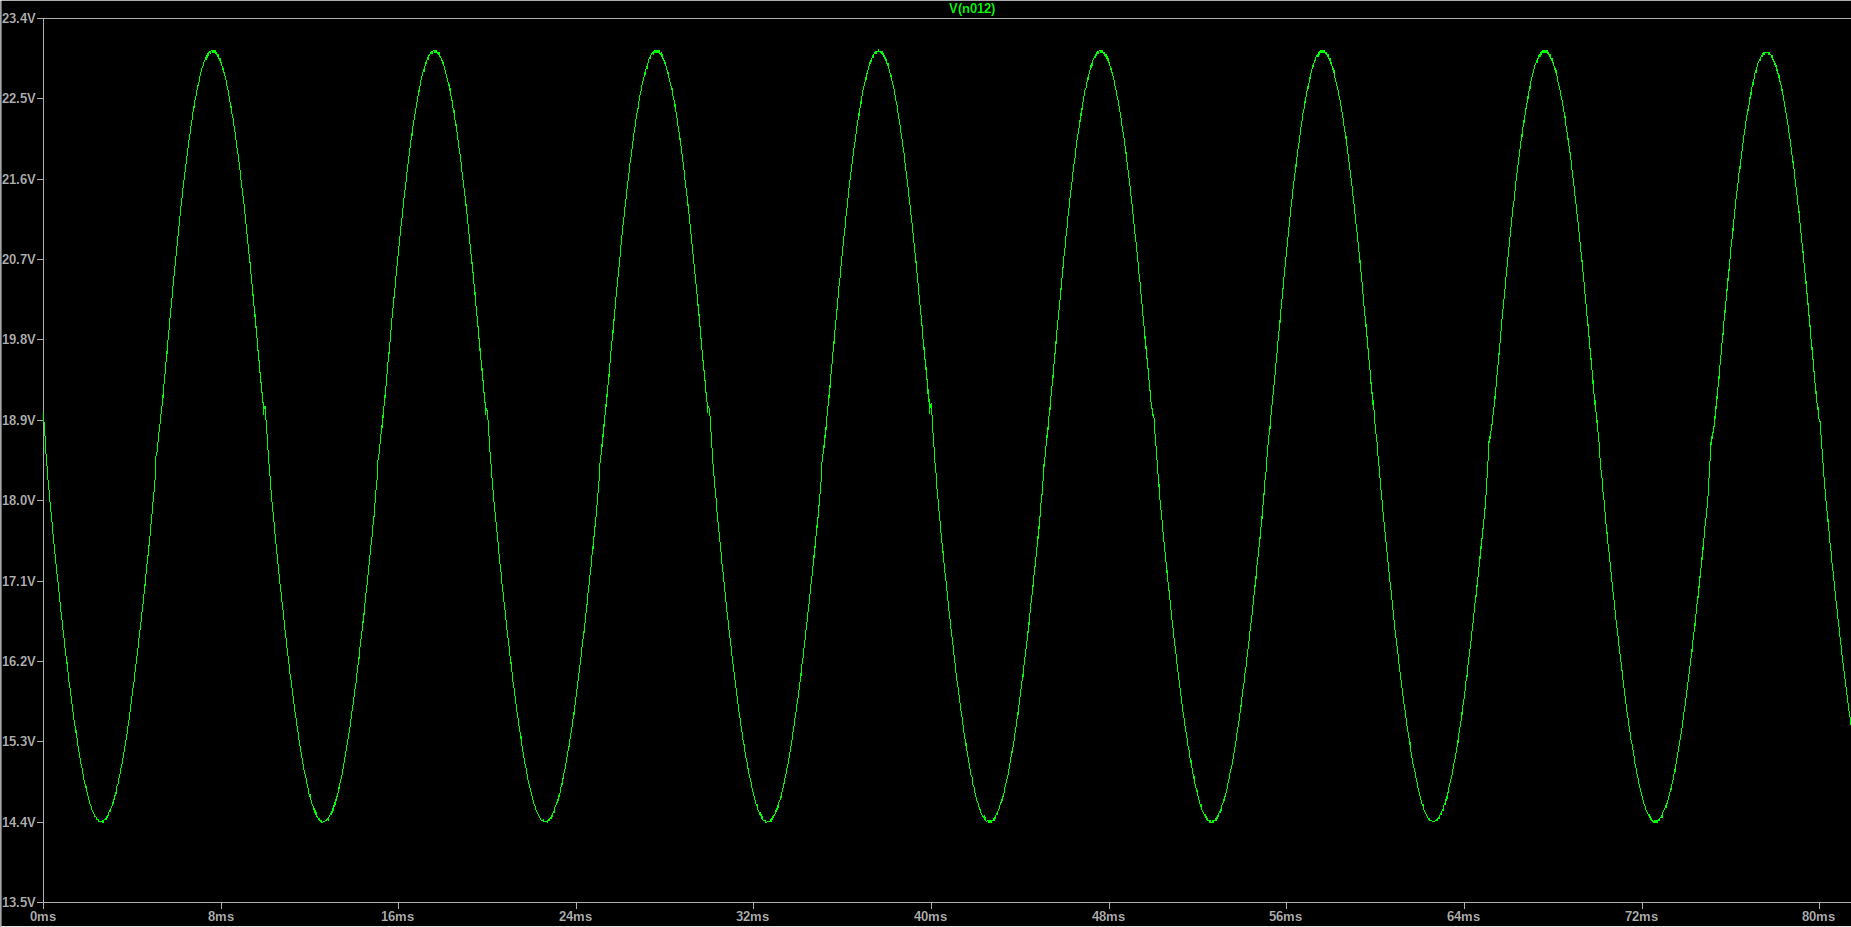
\includegraphics[width = \textwidth]{Vout_sigma_delta_100Hz.png}
	\caption{Sygnał odtworzony z sygnału  PDM ze wzmacniacza klasy d z modulatorem sigma-delta}
 \end{figure}

 \begin{figure} [H]
	\centering
	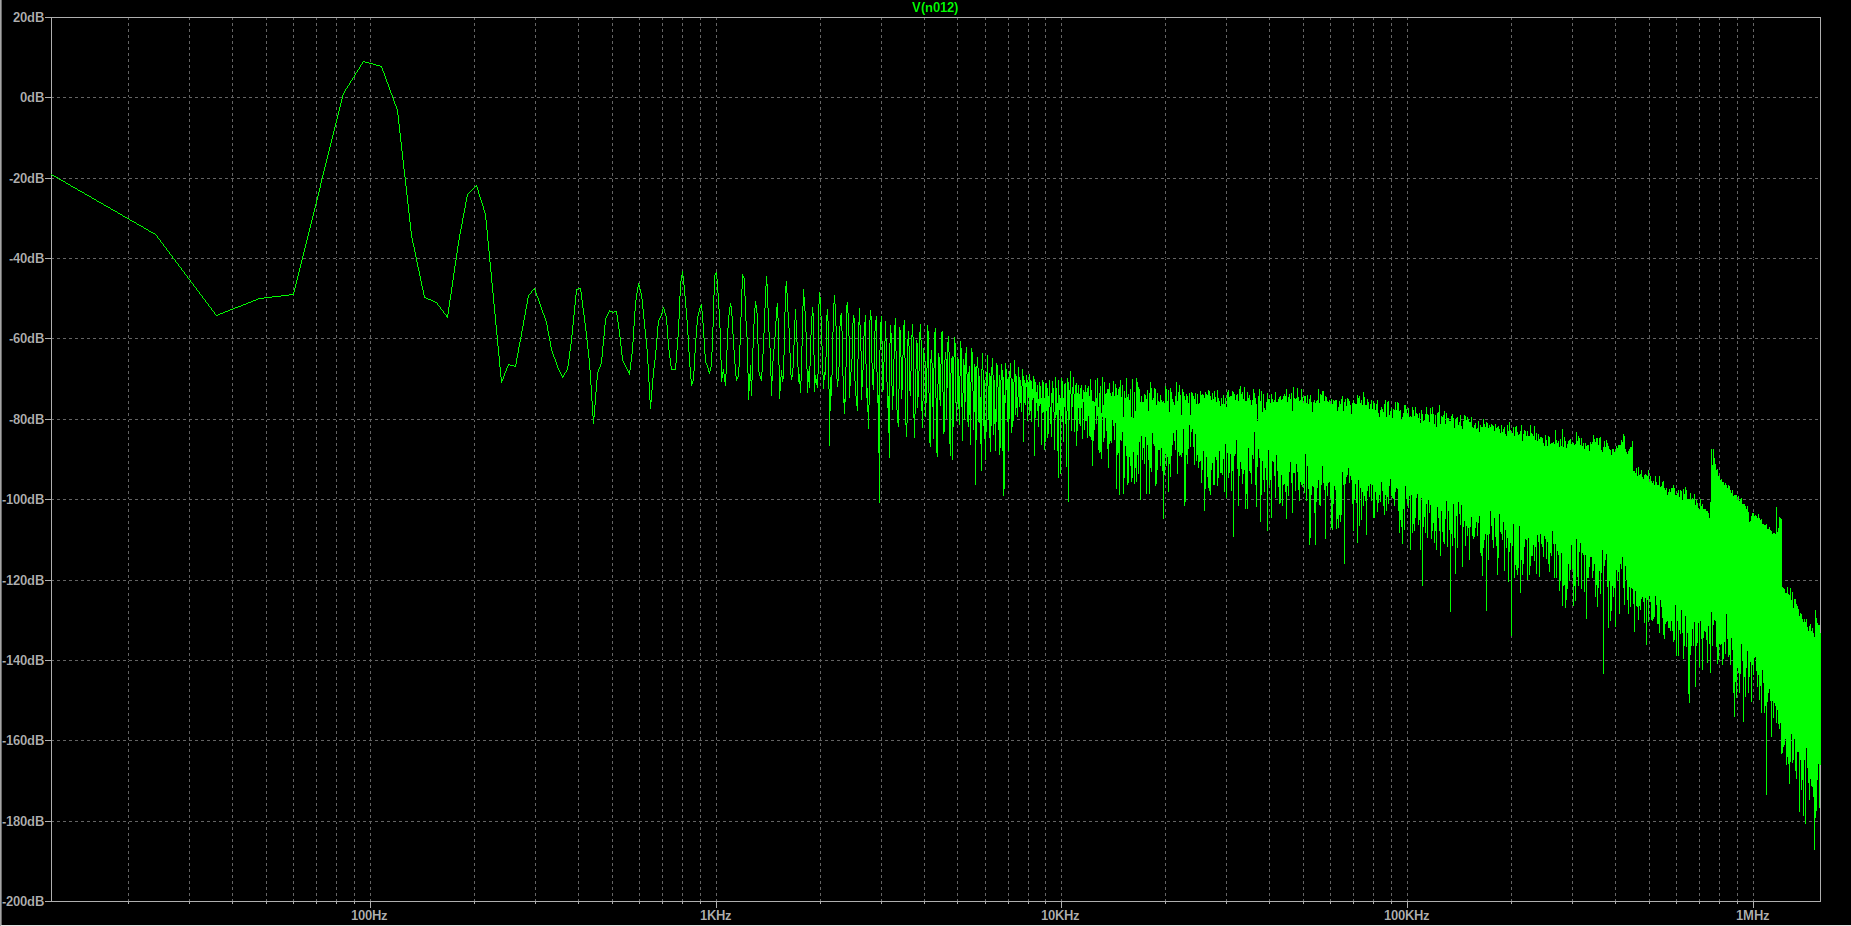
\includegraphics[width = \textwidth]{widmo_sigma_deltrat_100hz_2Vpp.png}
	\caption{Widmo sygnału odtworzonego ze wzmacniacza klasy D z modulatorem sigma delta}
 \end{figure}

 \begin{figure} [H]
	\centering
	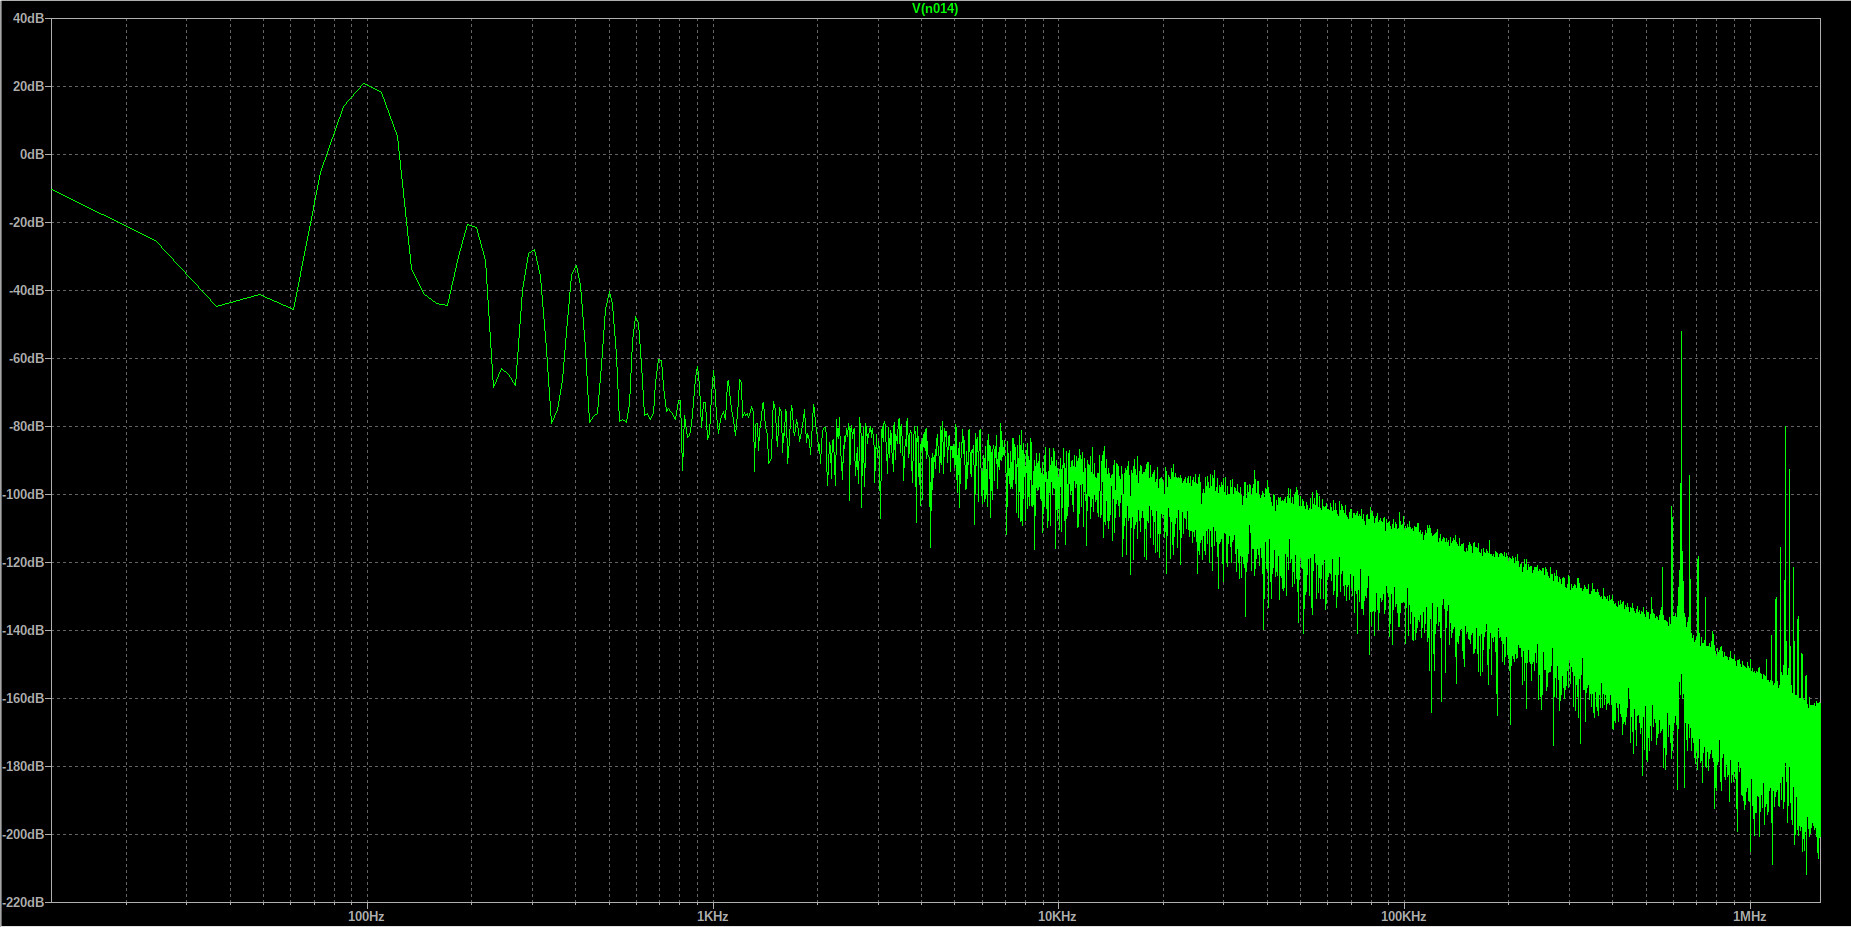
\includegraphics[width = \textwidth]{widmo_sygnału_comp_100hz_2Vpp.png}
	\caption{Widmo sygnału odtworzonego ze wzmacniacza klasy D z komparaotrem}
 \end{figure}
\subsection{Testy średnich częstotliwości $f_{in} = 1kHz.$}
Ze względu na to, że lepiej byłoby zaprezenotwać na żywo wyniki odtworzenia sygnału - a to jest projekt zaliczeniowy, pomienięto wstawianie obrazków
odtworzonego sygnału i wstawiono tylko widma.
\begin{figure} [H]
	\centering
	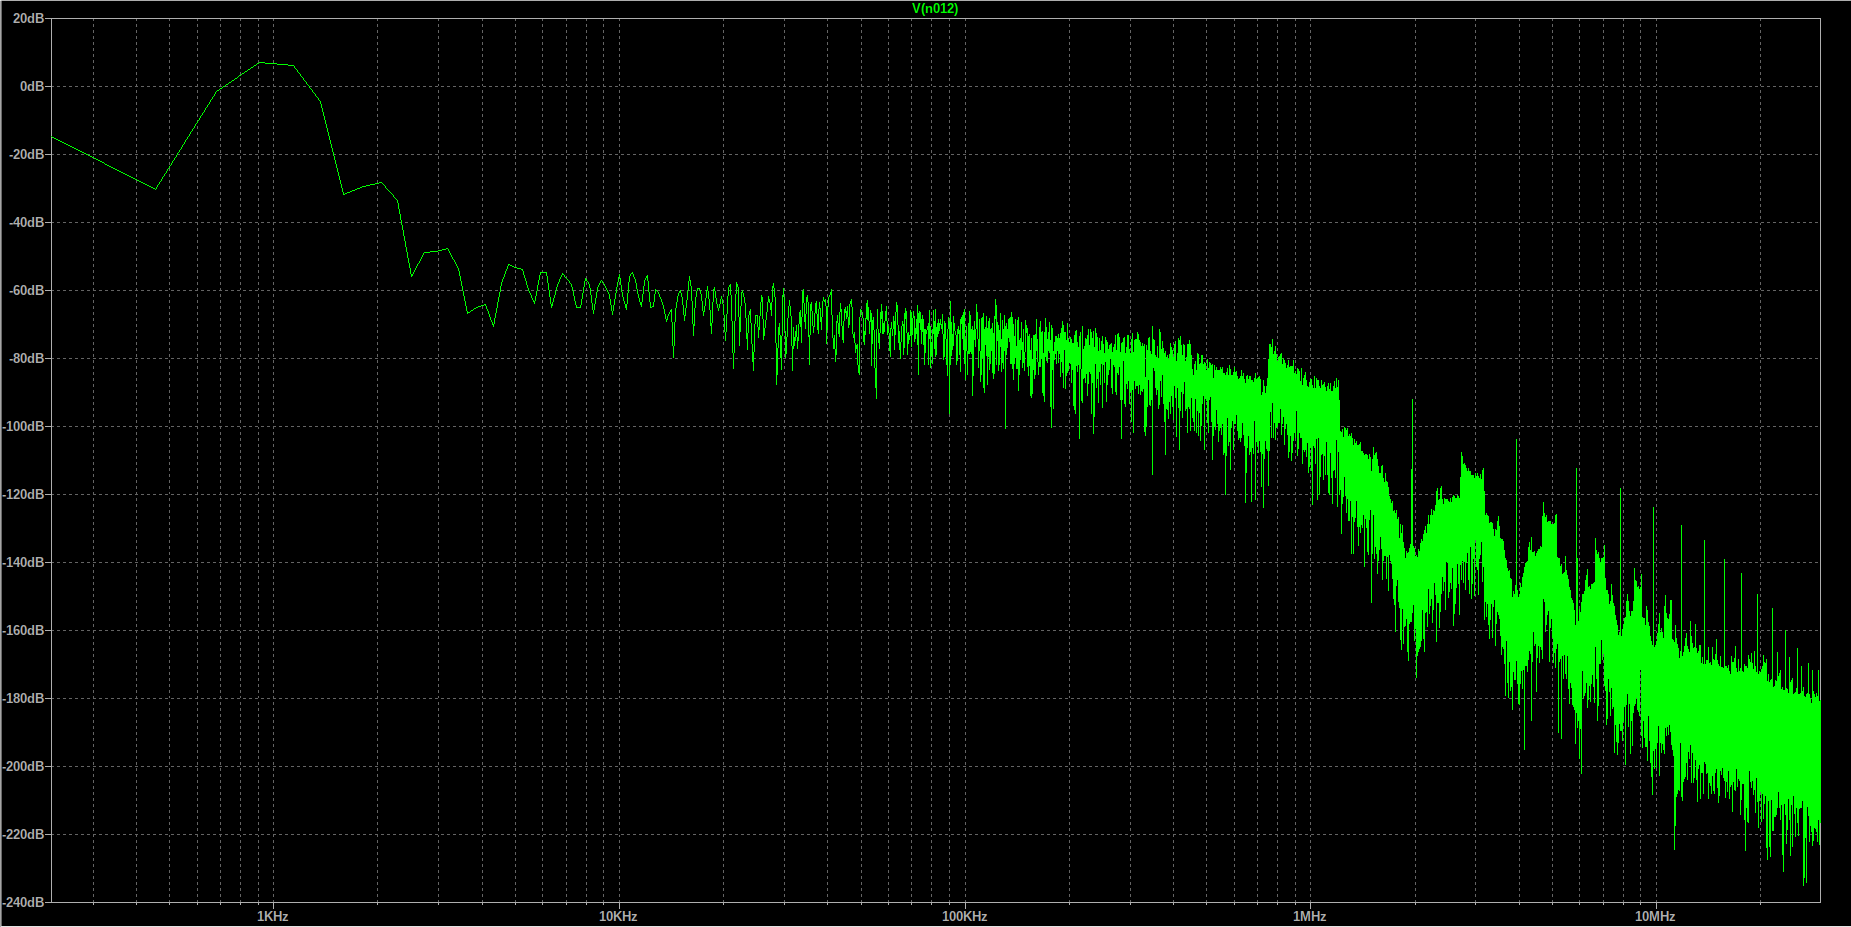
\includegraphics[width = \textwidth]{widmo_sigma_delta_1khz.png}
	\caption{Widmo sygnału odtworzonego ze wzmacniacza klasy D z modulatorem sigma delta}
 \end{figure}

 \begin{figure} [H]
	\centering
	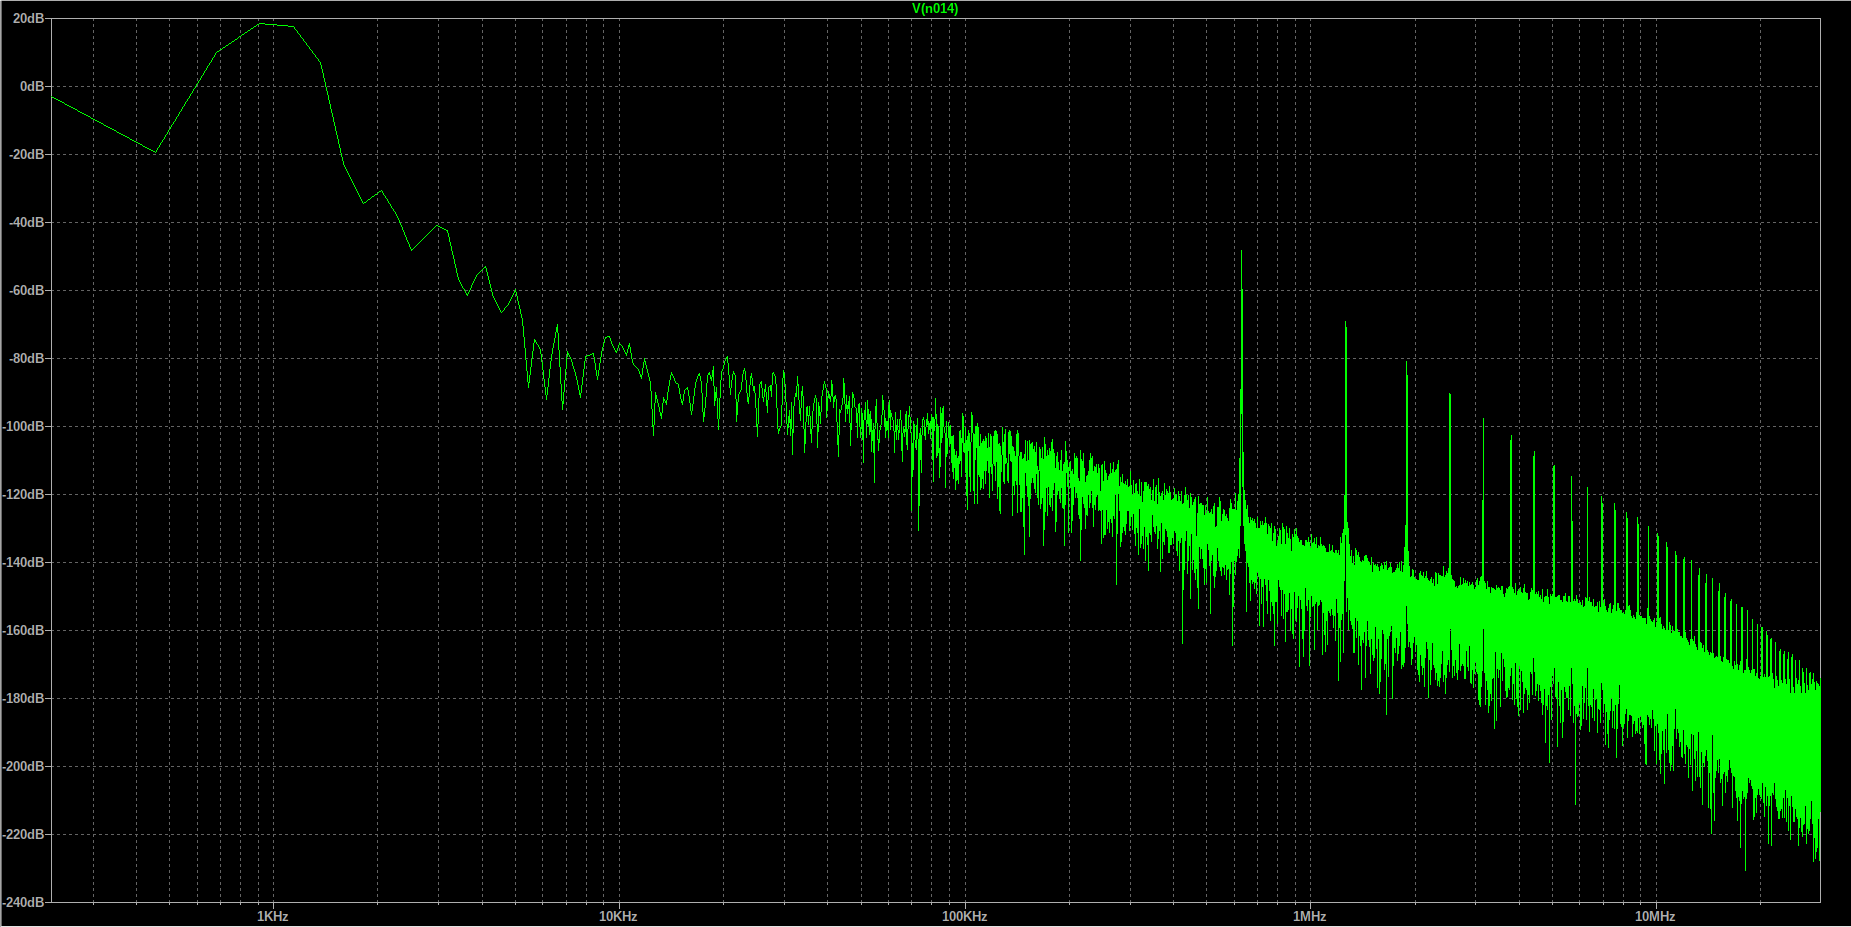
\includegraphics[width = \textwidth]{widmo_komp_1khz.png}
	\caption{Widmo sygnału odtworzonego ze wzmacniacza klasy D z komparatorem}
 \end{figure}

\subsection{Testy wysokich częstotliwości $f_{in} = 10kHz.$}
\begin{figure} [H]
	\centering
	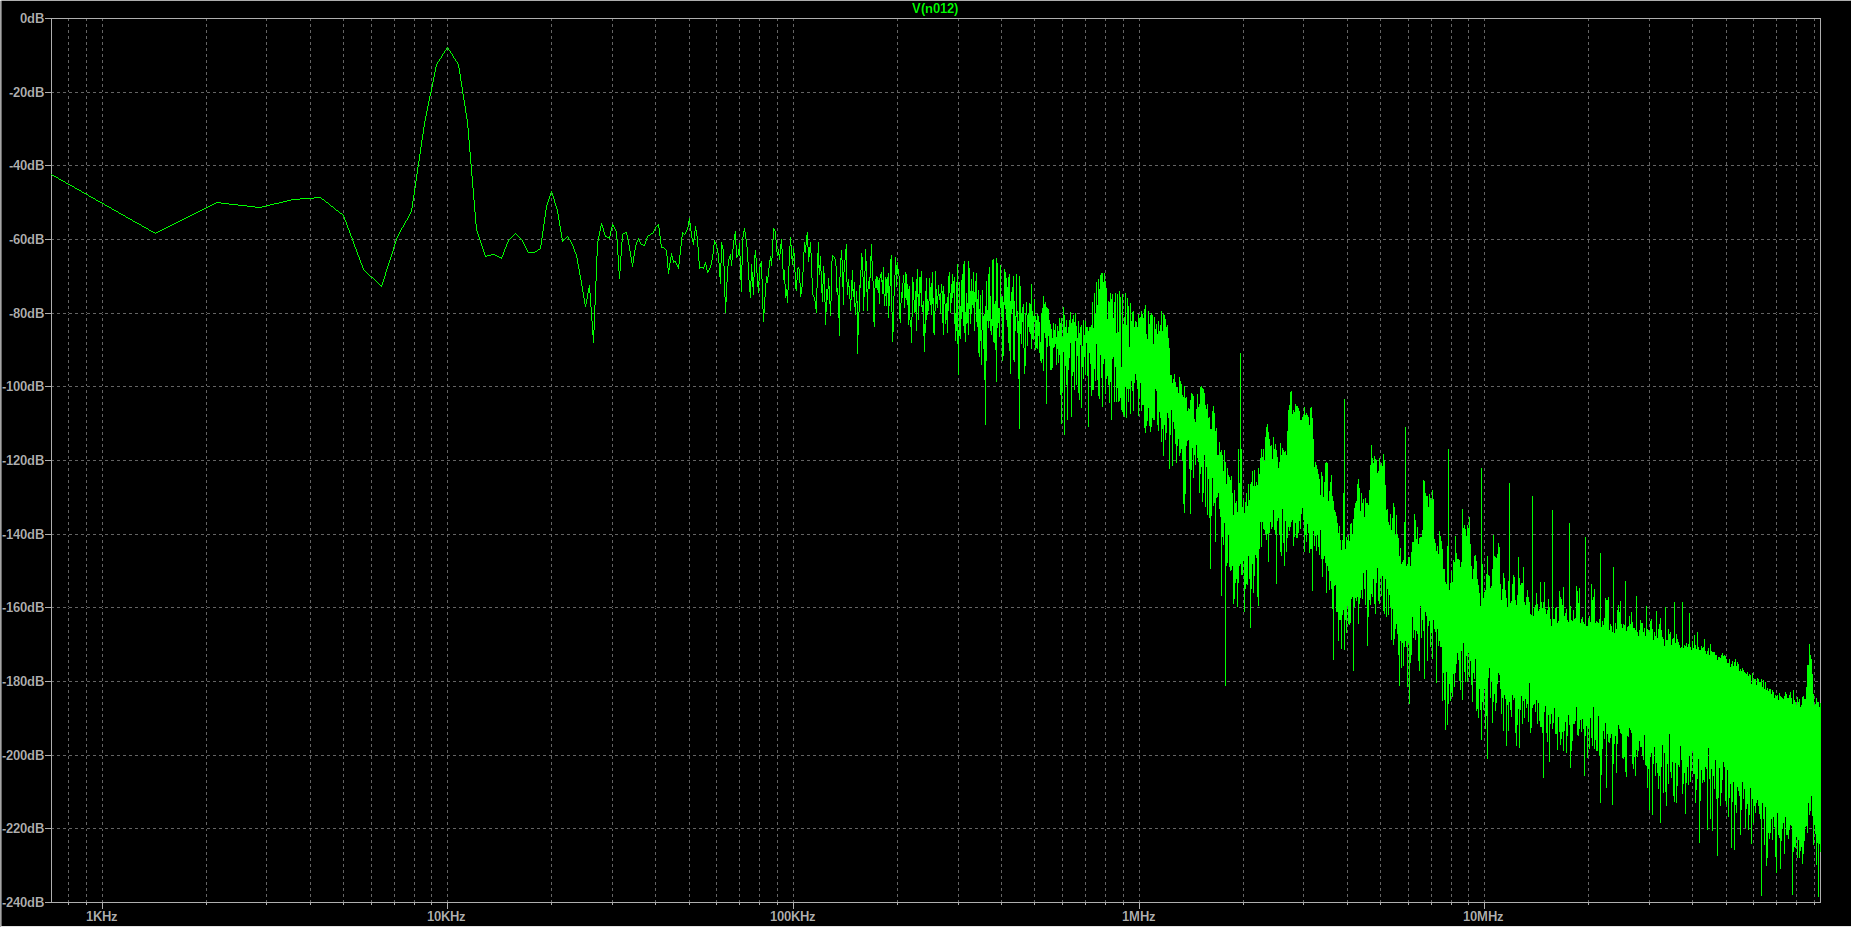
\includegraphics[width = \textwidth]{widmo_sugma_delta_10k.png}
	\caption{Widmo sygnału odtworzonego ze wzmacniacza klasy D z modulatorem sigma delta}
 \end{figure}

 \begin{figure} [H]
	\centering
	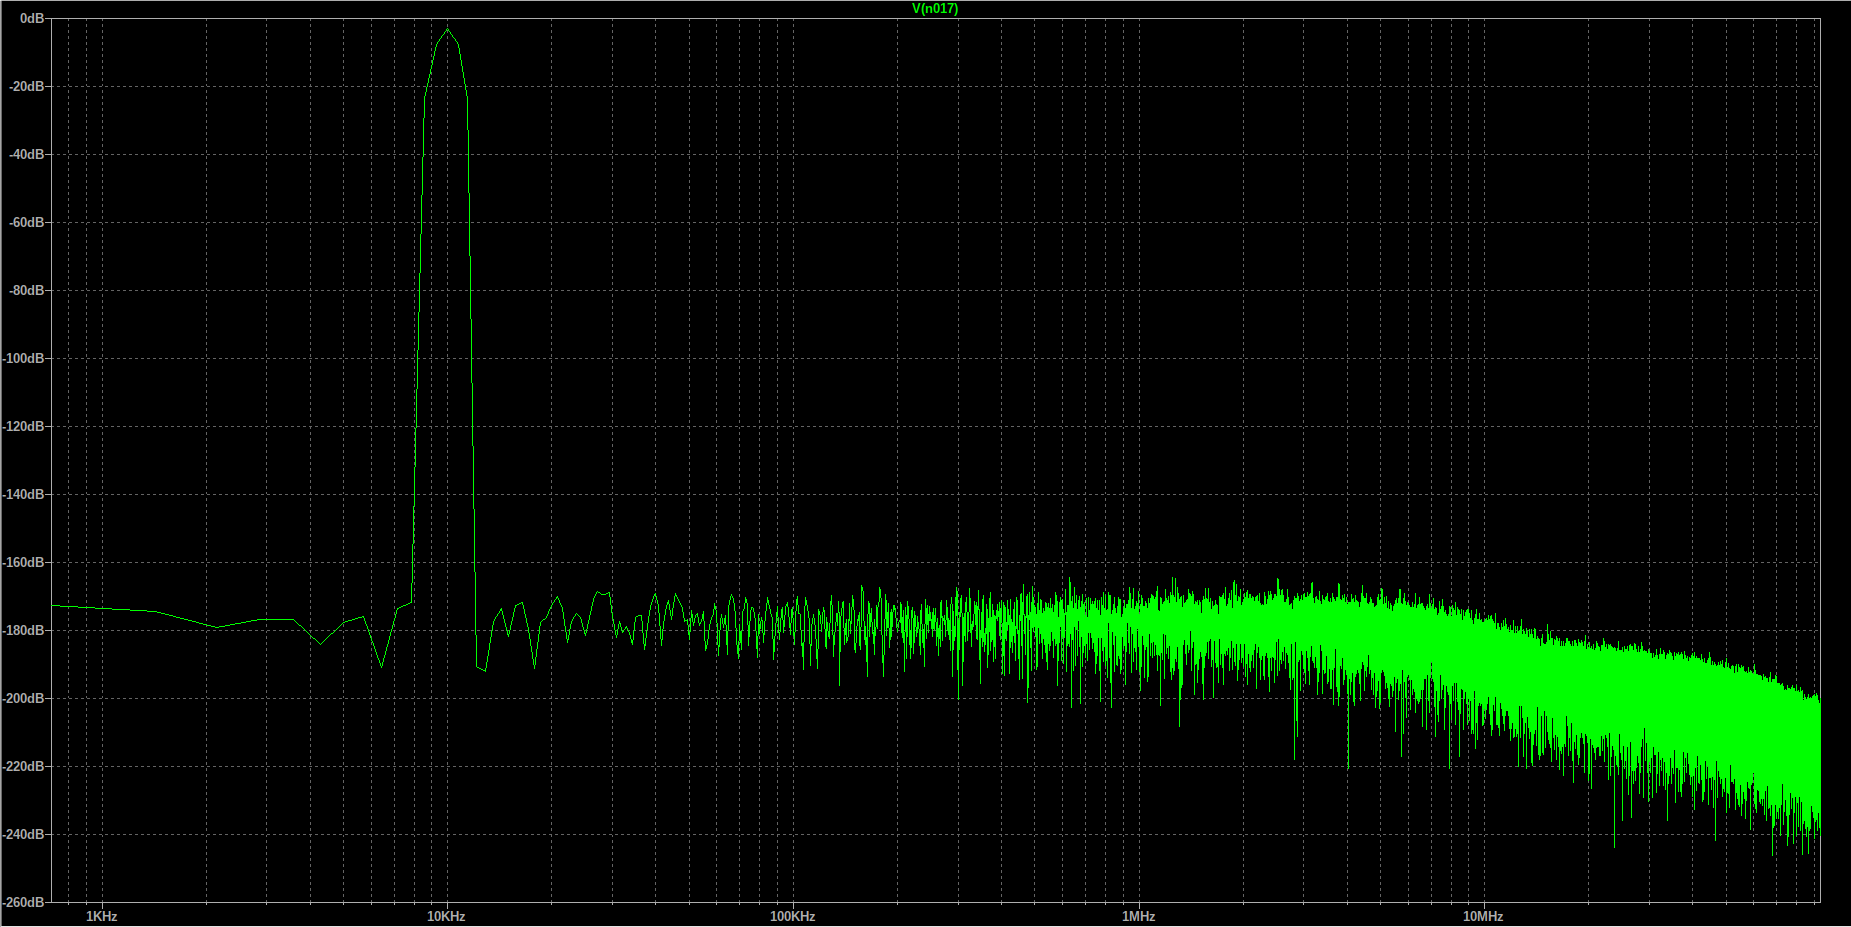
\includegraphics[width = \textwidth]{widmo_comp_10khz.png}
	\caption{Widmo sygnału odtworzonego ze wzmacniacza klasy D z komparatorem}
 \end{figure}
\section{Zakres zastosowania poszczególnych układów}
Obydwa układy znajdą zastosowanie jako wzmacniacze dużych mocy w sektorze audio. Wzmacniacz ze stopniem wejcsciowym z modulatorem Sigma-delta lepiej sobie radzi 
z odfiltrowywaniem harmonicznych i śmieci dla małych i śrenich częstotliwości.
\section{Spodziewane możliwości rozwoju projektu} 
Prawdopodobnie kolejnym krokiem byłoby przneiesienie implementacji w LTSpice na wykonanie projektu płytki w Altiumie.
\end{document}